%% LyX 2.3.7 created this file.  For more info, see http://www.lyx.org/.
%% Do not edit unless you really know what you are doing.
\documentclass[english]{article}
\usepackage[T1]{fontenc}
\usepackage[latin9]{inputenc}
\usepackage{array}
\usepackage{float}
\usepackage{url}
\usepackage{amsmath}
\usepackage{graphicx}

\makeatletter

%%%%%%%%%%%%%%%%%%%%%%%%%%%%%% LyX specific LaTeX commands.
%% Because html converters don't know tabularnewline
\providecommand{\tabularnewline}{\\}

%%%%%%%%%%%%%%%%%%%%%%%%%%%%%% Textclass specific LaTeX commands.
\newcommand{\lyxaddress}[1]{
	\par {\raggedright #1
	\vspace{1.4em}
	\noindent\par}
}

\makeatother

\usepackage{babel}
\usepackage{listings}
\renewcommand{\lstlistingname}{Listing}

\begin{document}
\title{OPTIMUS: a multidimensional global optimization package}
\author{Ioannis G. Tsoulos\thanks{Corresponding author. Email: itsoulos@uoi.gr},
Vasileios Charilogis}
\maketitle

\lyxaddress{Department of Informatics and Telecommunications, University of Ioannina,
Greece}
\begin{abstract}
A significant number of applications from many research areas can
be considered global optimization problems, such as applications in
the area of image processing, medical informatics, economic models,
etc. This paper presents a programming tool written in ANSI C++, which
researchers can use to formulate the problem to be solved and then
make use of the local and global optimization methods provided by
this tool to efficiently solve such problems. The main features of
the suggested software are: a) Coding of the objective problem in
a high level language such as ANSI C++ b) Incorporation of many global
optimization techniques to tackle the objective problem c)Parameterization
of global optimization methods using user-defined parameters.
\end{abstract}

\paragraph{Keywords: }

Global optimization; local optimization; stochastic methods; evolutionary
techniques; termination rules.

\section{Introduction}

The location of the global minimum for a continuous and differentiable
function $f:S\rightarrow R,S\subset R^{n}$ is formulated as
\begin{equation}
x^{*}=\mbox{arg}\min_{x\in S}f(x)\label{eq:eq1}
\end{equation}
where the set $S$ is defined as: 
\[
S=\left[a_{1},b_{1}\right]\otimes\left[a_{2},b_{2}\right]\otimes\ldots\left[a_{n},b_{n}\right]
\]
Methods that aim to locate the global minimum finds application in
problems from the area of economics \cite{globalecon1,globalecon2},
problems that appear very often in the area of physics \cite{global_physics1,global_physics2},
chemistry \cite{global_chemistry1,global_chemistry2}, common problems
from medicine \cite{global_med1,global_med2}, job scheduling problems
\cite{global_job1,global_job2}, water resources planning \cite{global_water1,global_water2},
network security problems \cite{global_network1,global_network2},
robotics \cite{global_robot1,global_robot2} etc. Also, global optimization
methods were used on some symmetry problems \cite{go_symmetry0,go_symmetry1,go_symmetry2}
as well as on inverse problems \cite{global_nonlinear1,global_nonlinear2,global_nonlinear3}.
In the relevant literature there are a number of global optimization
techniques, such as Adaptive Random Search methods \cite{go_adaptive1,go_adaptive2},
Controlled Random Search methods \cite{go_crs1,go_crs2}, Simulated
Annealing \cite{go_sa1,go_sa2,go_sa3}, Genetic algorithms \cite{go_ga1,go_ga2},
Ant Colony Optimization \cite{go_ant1,go_ant2}, Particle Swarm Optimization
\cite{go_pso1,go_pso2} etc. 

Due to the high importance of the global optimization problem, a variety
of hybrid optimization techniques have been proposed to handle the
global optimization problem, such as methods that combine Particle
Swarm Optimization and Genetic algorithms \cite{go_pso_genetic_hybrid1,go_pso_genetic_hybrid2},
combination of genetic algorithms and fuzzy logic classifier \cite{ga_fuzzy},
incorporation of genetic algorithm and the K-Means algorithm \cite{ga_kmeans},
combination of Particle Swarm Optimization method with Ant Colony
Optimization \cite{pso_aco1,pso_aco2,pso_aco3}, methods that combine
the Simplex method and Inductive search \cite{hybrid1} etc. Also,
many hybrid techniques combining local and global optimization have
been developed \cite{go_local1,go_local2,go_local3}.

Just a few recent application examples include an adaptive genetic
algorithm for crystal structure prediction \cite{genetic_physics1},
modeling of fusion plasma physics with genetic algorithms \cite{genetic_physics2},
usage of genetic algorithms for astroparticle physics studies \cite{genetic_physics3},
parameter extraction of solar cells using a Particle Swarm Optimization
method \cite{pso_physics1}, a new control approach of a a fleet of
Unmanned Aerial Vehicles using the method of Particle Swarm Optimization\cite{pso_physics2}
etc.

However, in most cases global optimization methods require a lot of
computing resources to implement both in memory and computing time.
Because of the large demands that global optimization methods have
on computing power, several techniques have been proposed such as
asynchronous methods \cite{async1,async2,async3}, parallel approaches
of the Multistart optimization method \cite{parallel-multistart,parallel-multistart2}
and also some methods that take advantage of modern parallel GPU architectures
\cite{gpu1,gpu2,gpu3}.

In this paper, a new integrated computing environment for performing
global optimization methods for multidimensional functions is presented
and analyzed in detail. In this computing environment, the programmer
can code the problem to be solved using a high-level programming language
such as C++. In addition to the objective function, the programmer
can also provide information that the objective problem should have
at the start of the optimization process and in addition can formulate
a series of actions that will take place after the optimization process
is finished. Subsequently, the researcher can formulate a strategy
to solve the problem. In this strategy, the researcher can choose
from a series of sampling methods, choose a global minimization method
established in the relevant literature and possibly some local minimization
method to improve the produced result. Similar software environments
can be found, such as the BARON software package \cite{baron} for
non convex optimization problems, the MERLIN optimization software
\cite{merlin} which is accompanied with the Merlin Control Language
compiler to guide the optimization course, the DEoptim software \cite{deoptim}
which is an R package implementing the differential evolution algorithm,
the PDoublePop optimization software \cite{pdoublepop} that implements
a parallel genetic algorithm for global optimization etc.

Also recently, some other optimization tools have been appeared such
as the Paradiseo \cite{paradiseo} implemented in C++ that mainly
contains evolutionary algorithms, the Pagmo software \cite{pagmo}
where a wide range of evolution algorithms are incorporated to solve
optimization problems and finally another approach for evolutionary
algorithms applied to optimization problems is the HeuristicLab freely
available from \url{https://dev.heuristiclab.com/trac.fcgi/}, used
mainly for online optimization. In the proposed software, the user
can write the required objective function in simple C++ and then choose
from a wide range of global optimization methods the most suitable
one for finding the global minimum. Furthermore, in the proposed software
the user can parameterize the local minimization method to be used
as well as the termination method to be used for the successful termination
of the technique. In addition, it is possible for the user to create
his own global minimization method from scratch using the programming
tools of the Optimums libraries.

The rest of this article is structured as follows: in section \ref{sec:Software}
the proposed software is outlined in detail, in section \ref{sec:Experiments}
some experiments are conducted to show the effectiveness of the proposed
software and finally in section \ref{sec:Conclusions} some conclusions
and guidelines for future work are presented.

\section{Software\label{sec:Software}}

The suggested software is entirely coded in ANSI C++, using the freely
available QT programming library, which can be downloaded from \url{https://qt.io}
(accessed on 8 February 2023). The researcher should code the objective
function and a number of other mandatory functions in the C++ programming
language. Also, the researcher should provide the dimension of the
objective function as well as the bound of the function (equation
\ref{eq:eq1}). Subsequently, the user can select a global optimization
method to apply to the problem from a wide range of available methods.
Also, the user can extend the series of methods by adding any new
method that follows the guidelines of the software.\textbf{ }In the
following subsections, the installation process of the suggested software
will be analyzed and a complete example of running an objective problem
will be given.

\subsection{Installation }

At the present time, the software package can only be installed on
computers with the Linux operating system, but in the future it will
be able to be installed on other systems as well. The instructions
to install the package on a computer are as follows:
\begin{enumerate}
\item Download and install the QT programming library from \url{https://qt.io }.
In most Linux distributions this library can be made available from
the relevant distribution repositories.
\item Download and unzip the software from \url{https://github.com/itsoulos/OPTIMUS}.
\item Set the \emph{OPTIMUSPATH} environment variable pointing at the installation
directory of OPTIMUS e.g. OPTIMUSPATH=/home/user/OPTIMUS/, where user
is the user name in the Linux operating system. This step is necessary
so that the compiler can locate the necessary files during compilation.
\item Set the \emph{LD\_LIBRAPY\_PATH} to include the OPTIMUS/lib subdirectory
e.g. \\
LD\_LIBRAPY\_PATH=\$LD\_LIBRAPY\_PATH:\$OPTIMUSPATH/lib/:
\item Issue the command: cd \$OPTIMUSPATH 
\item Execute the compilation script:\emph{ ./compile.sh }
\end{enumerate}
The compilation will take some minutes in most modern computer systems
and when the compilation is complete, the \emph{lib} folder will contain
the supported global optimization methods in the form of shared libraries,
the \emph{PROBLEMS} folder will contain a number of example optimization
problems from the relevant literature, and the \emph{bin} folder will
contain the main executable of the software named \emph{OptimusApp}.
This executable can be used to apply global optimization techniques
to objective problems.

\subsection{Implemented global optimization methods }

In the following, the global optimization methods present in the proposed
software are presented. In most of them, a local optimization method
is applied after their end in order to find the global minimum with
greater reliability. In the proposed software, each implemented global
optimization method has a set of parameters that can determine the
global optimization path and the effectiveness of the method. For
example, the genetic algorithm contains parameters such as the number
of chromosomes or the maximum number of generations allowed. In addition,
to make the optimization process easier, each method has been assigned
a symbolic name, such as pso for particle swarm optimization. The
implemented global optimization methods are:
\begin{enumerate}
\item Differential Evolution. The differential evolution method is included
in the software as suggested by Storn\cite{de_main_paper} and denoted
as \textbf{de}. This global optimization technique has been widely
used in areas such as data mining applications \cite{de_datamining,de_symmetry1},
material design problems \cite{de_symmetry3}, feature selection \cite{de_symmetry6},
clustering methods \cite{de_symmetry7} etc.
\item Improved Differential Evolution. The modified Differential Evolution
method as suggested by Charilogis et al \cite{gende} is implemented
and denoted as \textbf{gende}. This modification of the Differential
Evolution method introduces two variations: a new asymptotic stopping
rule and a new scheme for a critical parameter of the method. 
\item Parallel Differential Evolution. A parallel implementation of the
Differential Evolution method as suggested in \cite{parallelDe} is
considered with the name \textbf{ParallelDe}. This parallel technique
divides the total work into a number of available parallel computing
units, and in each unit an independent Differential Evolution method
is executed. The parallelization is performed using the OpenMP programming
library \cite{openMp}.
\item Double precision genetic algorithm. A modified genetic algorithm \cite{doublepop_tsoulos}
is included in the software and it is denoted as \textbf{DoubleGenetic}.
Genetic algorithms are typical representatives of evolutionary techniques
with many applications such as scheduling problems \cite{genetic1},
the vehicle routing problem \cite{genetic2}, combinatorial optimization
\cite{genetic3}, architectural design etc \cite{genetic4}.
\item Integer precision genetic algorithm. The method denoted as \textbf{IntegerGenetic}
is a copy of the \textbf{DoubleGenetic} method, but with the usage
of integer values as chromosomes. This global optimization method
is ideal for problems such as the TSP problem \cite{tsp1,tsp2}, path
planning \cite{pathPlanning}, Grammatical Evolution applications
\cite{ge} etc.
\item Improved Controlled Random Search. An improved version of Controlled
Random Search as suggested by Charilogis et al \cite{gcrs} is implemented
and it is denoted as \textbf{gcrs}. This variation modifies the original
method by adding a new sampling method, a new stochastic termination
rule and a periodical application of a local optimization procedure.
\item Particle Swarm Optimization. A PESO variant denoted as \textbf{Pso}
is also included in the software. The particle swarm optimization
method was applied successfully in a vast number of problems such
as parameter extraction of solar cells \cite{psoApp1}, crystal structure
prediction \cite{psoApp2}, molecular simulations \cite{psoApp3}
etc.
\item Improved Particle Swarm Optimization. The improved Particle Swarm
method as suggested by Charilogis and Tsoulos \cite{ipso}. The implemented
method is denoted as \textbf{iPso}. The original Particle Swarm Optimization
method is enhanced using a new inertia calculation mechanism as well
as a novel termination method.
\item Multistart. A simple method that initiates local searches from different
initial points is also implemented in the software. Despite its simplicity,
the multistart method has been applied on many problems, such as the
TSP problem\textbf{ }\cite{multistart-tsp}, the vehicle routing problem
\cite{multistart-vehicle}, the facility location problem \cite{multistart_fac},
the maximum clique problem \cite{multistart_clique}, the maximum
fire risk insured capital problem \cite{multistart_fire}, aerodynamic
problems \cite{multistart-aero} etc
\item Topographical Multi level single linkage. This method is proposed
by Ali et al \cite{tmlsl} and it is denoted as \textbf{Tmlsl} in
the implementation. 
\item The MinCenter method. In the software presented here, another multistart
method has been included, which forms, with the use of the K-Means
algorithm for clustering purposes, the regions of attraction for the
local minima of the objective problem. This method is denoted as \textbf{MinCenter}
and it was originally published by Charilogis and Tsoulos \cite{mincenter}.
\item NeuralMinimizer. A novel method that incorporates Radial Basis Functions
(RBF)\cite{rbf_main1} to create an estimation of the objective function
introduced in \cite{neuralMinimizer} is implemented and denoted by
the name \textbf{NeuralMinimizer}.
\end{enumerate}

\subsection{Implemented local optimization methods}

All global optimization methods can be enhanced by applying a local
minimization method after they are terminated. The parameter used
to determine the used local optimization procedure is the $--$localsearch\_method
parameter. The implemented local optimization methods are the following:
\begin{enumerate}
\item The \textbf{bfgs} method. The Broyden--Fletcher--Goldfarb--Shanno
(BFGS) algorithm was implemented using a variant of Powell \cite{powell}.
\item The \textbf{lbfgs} method. The limited memory BFGS method \cite{lbfgs}
is implemented as an approximation of the BFGS method using a limited
amount of computer memory. This local search procedure is ideal for
objective functions of higher dimensions.
\item The Gradient descent method. This method is denoted as \textbf{gradient}
in the software and implements the Gradient Descent local optimization
procedure. This local search procedure is used in various problems
such as neural network training \cite{gradient1}, image registration
\cite{gradient2} etc.
\item The \textbf{adam} method. The adam local optimizer \cite{Adam} is
implemented also.
\item The Nelder Mead method. The Nelder - Mead simplex procedure for local
optimization \cite{nelderMead} is also included in the software and
it is denoted as \textbf{nelderMead}.
\item Hill climbing. The hill climbing local search procedure denoted as
\textbf{hill} is also implemented. The method has been used in various
fields, such as design of photovoltaic power systems \cite{hill1},
load balancing in cloud computing \cite{hill2} etc. 
\end{enumerate}

\subsection{Objective problem deployment }

The objective problem must be coded in the C++ programming language.
The programmer must describe in detail the problem to be solved and
must provide the software with detailed information about the dimension
of the problem, the value limits of the variables of the problem,
the objective function and also the derivative of the function. If
the analytical derivative is not available or difficult to calculate
then the programmer can program it using finite differences or use
some automatic differentiation software, such as the Adept software
\cite{adept}.

\subsubsection{Objective function coding}

Figure \ref{fig:A-typical-representation} shows an example of objective
function. The figure show also the required functions by the proposed
software. This code is used for the minimization of the Rastrigin
function defined as:
\[
f(x)=x_{1}^{2}+x_{2}^{2}-\cos\left(18x_{1}\right)-\cos\left(18x_{2}\right)
\]
with $x\in[-1,1]^{2}$. The functions shown in the figure \ref{fig:A-typical-representation}
have the following meaning:
\begin{enumerate}
\item \textbf{void} init(QJsonObject data). The function init() is called
before the objective function is executed and its purpose is to pass
parameters from the execution environment to the objective function.
For example, for the Lennard Jones potential \cite{originalJones},
the user can pass the number of atoms in the potential using an assignment
as follows\\
\begin{lstlisting}
        natoms=data["natoms"].toString().toInt(); 
\end{lstlisting}
If the objective problem does not need a parameter, then this function
can be empty.
\item \textbf{int} getDimension(). This function returns the dimension of
the objective problem.
\item \textbf{void}    getmargins(vector<Interval> \&x). The getmargins()
functions returns in the vector x the bounds of the objective problem.
The class Interval is a simple class located in the folder \emph{PROBLEMS}
of the distribution, that represents double precision intervals eg
the value $[2,4${]} is an interval with left bound the value 2 and
right bound the value 4.
\item \textbf{double}	funmin(vector<\textbf{double}> \&x). This function
returns the objective problem $f(x)$ for a given point $x$. The
number of elements of the vector x must be the same in number as the
return value of the function getDimension().
\item \textbf{void}    granal(vector<\textbf{double}> \&x,vector<\textbf{double}>
\&g). This functions stores in vector g the gradient $\nabla f(x)$
for a given point x.
\item QJsonObject  done(vector<\textbf{double}> \&x). This function is executed
after the objective function optimization process is completed. The
point x is the global minimum for the function $f(x)$. This function
can be used in various cases, such as to generate a graph after the
optimization is finished or even in the case of artificial neural
networks \cite{nn1,nn2} to apply the resulting trained network to
the test set of the problem.
\end{enumerate}
\begin{figure}
\caption{A typical representation of an objective problem, suitable for the
OPTIMUS programming tool.\label{fig:A-typical-representation}}

\begin{lstlisting}[language={C++}]
# include <math.h> 
# include <interval.h> 
# include <vector> 
# include <stdio.h> 
# include <iostream> 
# include <QJsonObject> 
using namespace std;
extern "C" {
void    init(QJsonObject data) {
}
int	getdimension() { 	
	return 2; 
} 
void    getmargins(vector<Interval> &x) {         
  for(int i=0;i<x.size();i++)                 
	x[i]=Interval(-1,1); 
}
double	funmin(vector<double> &x) {    
	return (x[0]*x[0])+(x[1]*x[1])-cos(18.0*x[0])-cos(18.0*x[1]); 
}
void    granal(vector<double> &x,vector<double> &g) {       
	g[0]=2.0*x[0]+18.0*sin(18.0*x[0]);       
	g[1]=2.0*x[1]+18.0*sin(18.0*x[1]); 
}
QJsonObject    done(vector<double> &x) {     
return QJsonObject(); 
}
} 
\end{lstlisting}
\end{figure}


\subsubsection{Objective function compilation }

In order to build the objective function the user should create an
accompaniment project file as demonstrated in Figure \ref{fig:proFile}.
The first line of this project file determines the a shared library
will be build by the compilation. The second line lists the number
of source files that will be compiled and the last line contains the
names of the header files. The software incorporates the utility qmake
of the QT library to compile the objective function. The compilation
is performed with the following series of commands in the terminal:
\begin{enumerate}
\item qmake \emph{file.pro}
\item make
\end{enumerate}
where\emph{ file.pro }stands for the name of the project file. The
final outcome of this compilation will be the shared library \emph{libfile.so}

\begin{figure}
\caption{The associated project file for the Rastrigin problem.\label{fig:proFile}}

\begin{lstlisting}
TEMPLATE=lib 
SOURCES+=rastrigin.cc interval.cpp
HEADERS += interval.h
\end{lstlisting}
\end{figure}


\subsubsection{Objective function execution}

A full working command for the Rastrigin problem using the utility
program \emph{OptimusApp} is shown below

\begin{lstlisting}[language={C++},basicstyle={\normalsize},breaklines=true,literate={{-}{-}1}]
./OptimusApp --filename=librastrigin.so --opt_method=Pso\ --pso_particles=100 --pso_generations=10\  
    --localsearch_method=bfgs
\end{lstlisting}
The parameters for the above command line are as follows:
\begin{enumerate}
\item The argument of the option $--$filename determines the objective
problem in shared library format.
\item The argument of the command line option $--$opt\_method sets the
used global optimization procedure. For this case, the Particle Swarm
Optimizer was used. 
\item The argument of the option $--$pso\_particles sets the number of
particles of the PESO optimizer.
\item The argument for the command line option $--$pso\_generations sets
the maximum number of generations allowed.
\item The argument $--$localsearch\_method sets the used local optimization
procedure, that will be applied on the best particle of the PESO procedure
when it finishes.
\end{enumerate}
The output of the previous command is shown in figure \ref{fig:rastrigin_output}.
As it is obvious, the global optimization method is quite close to
the global minimum of the function, which is -2. However with the
help of the local optimization method applied after its end, this
minimum is found with greater numerical accuracy. 

The main steps of a typical usage of the software have been also shown
in graphical format in Figure \ref{fig:optSteps}.

\begin{figure}[H]
\caption{Output for the minimization of the Rastrigin function using the PESO
optimizer.\label{fig:rastrigin_output}}

\begin{lstlisting}
Generation     1 value:   -1.7464048
Generation     2 value:   -1.8619942
Generation     3 value:   -1.8852439
Generation     4 value:   -1.9490074
Generation     5 value:   -1.9490074
Generation     6 value:   -1.9490074
Generation     7 value:   -1.9490074
Generation     8 value:   -1.9775267
Generation     9 value:   -1.9972928
Generation    10 value:   -1.9977027
Minimum:       -2.0000000000  Function calls:    1028
\end{lstlisting}
\end{figure}
\begin{figure}[H]
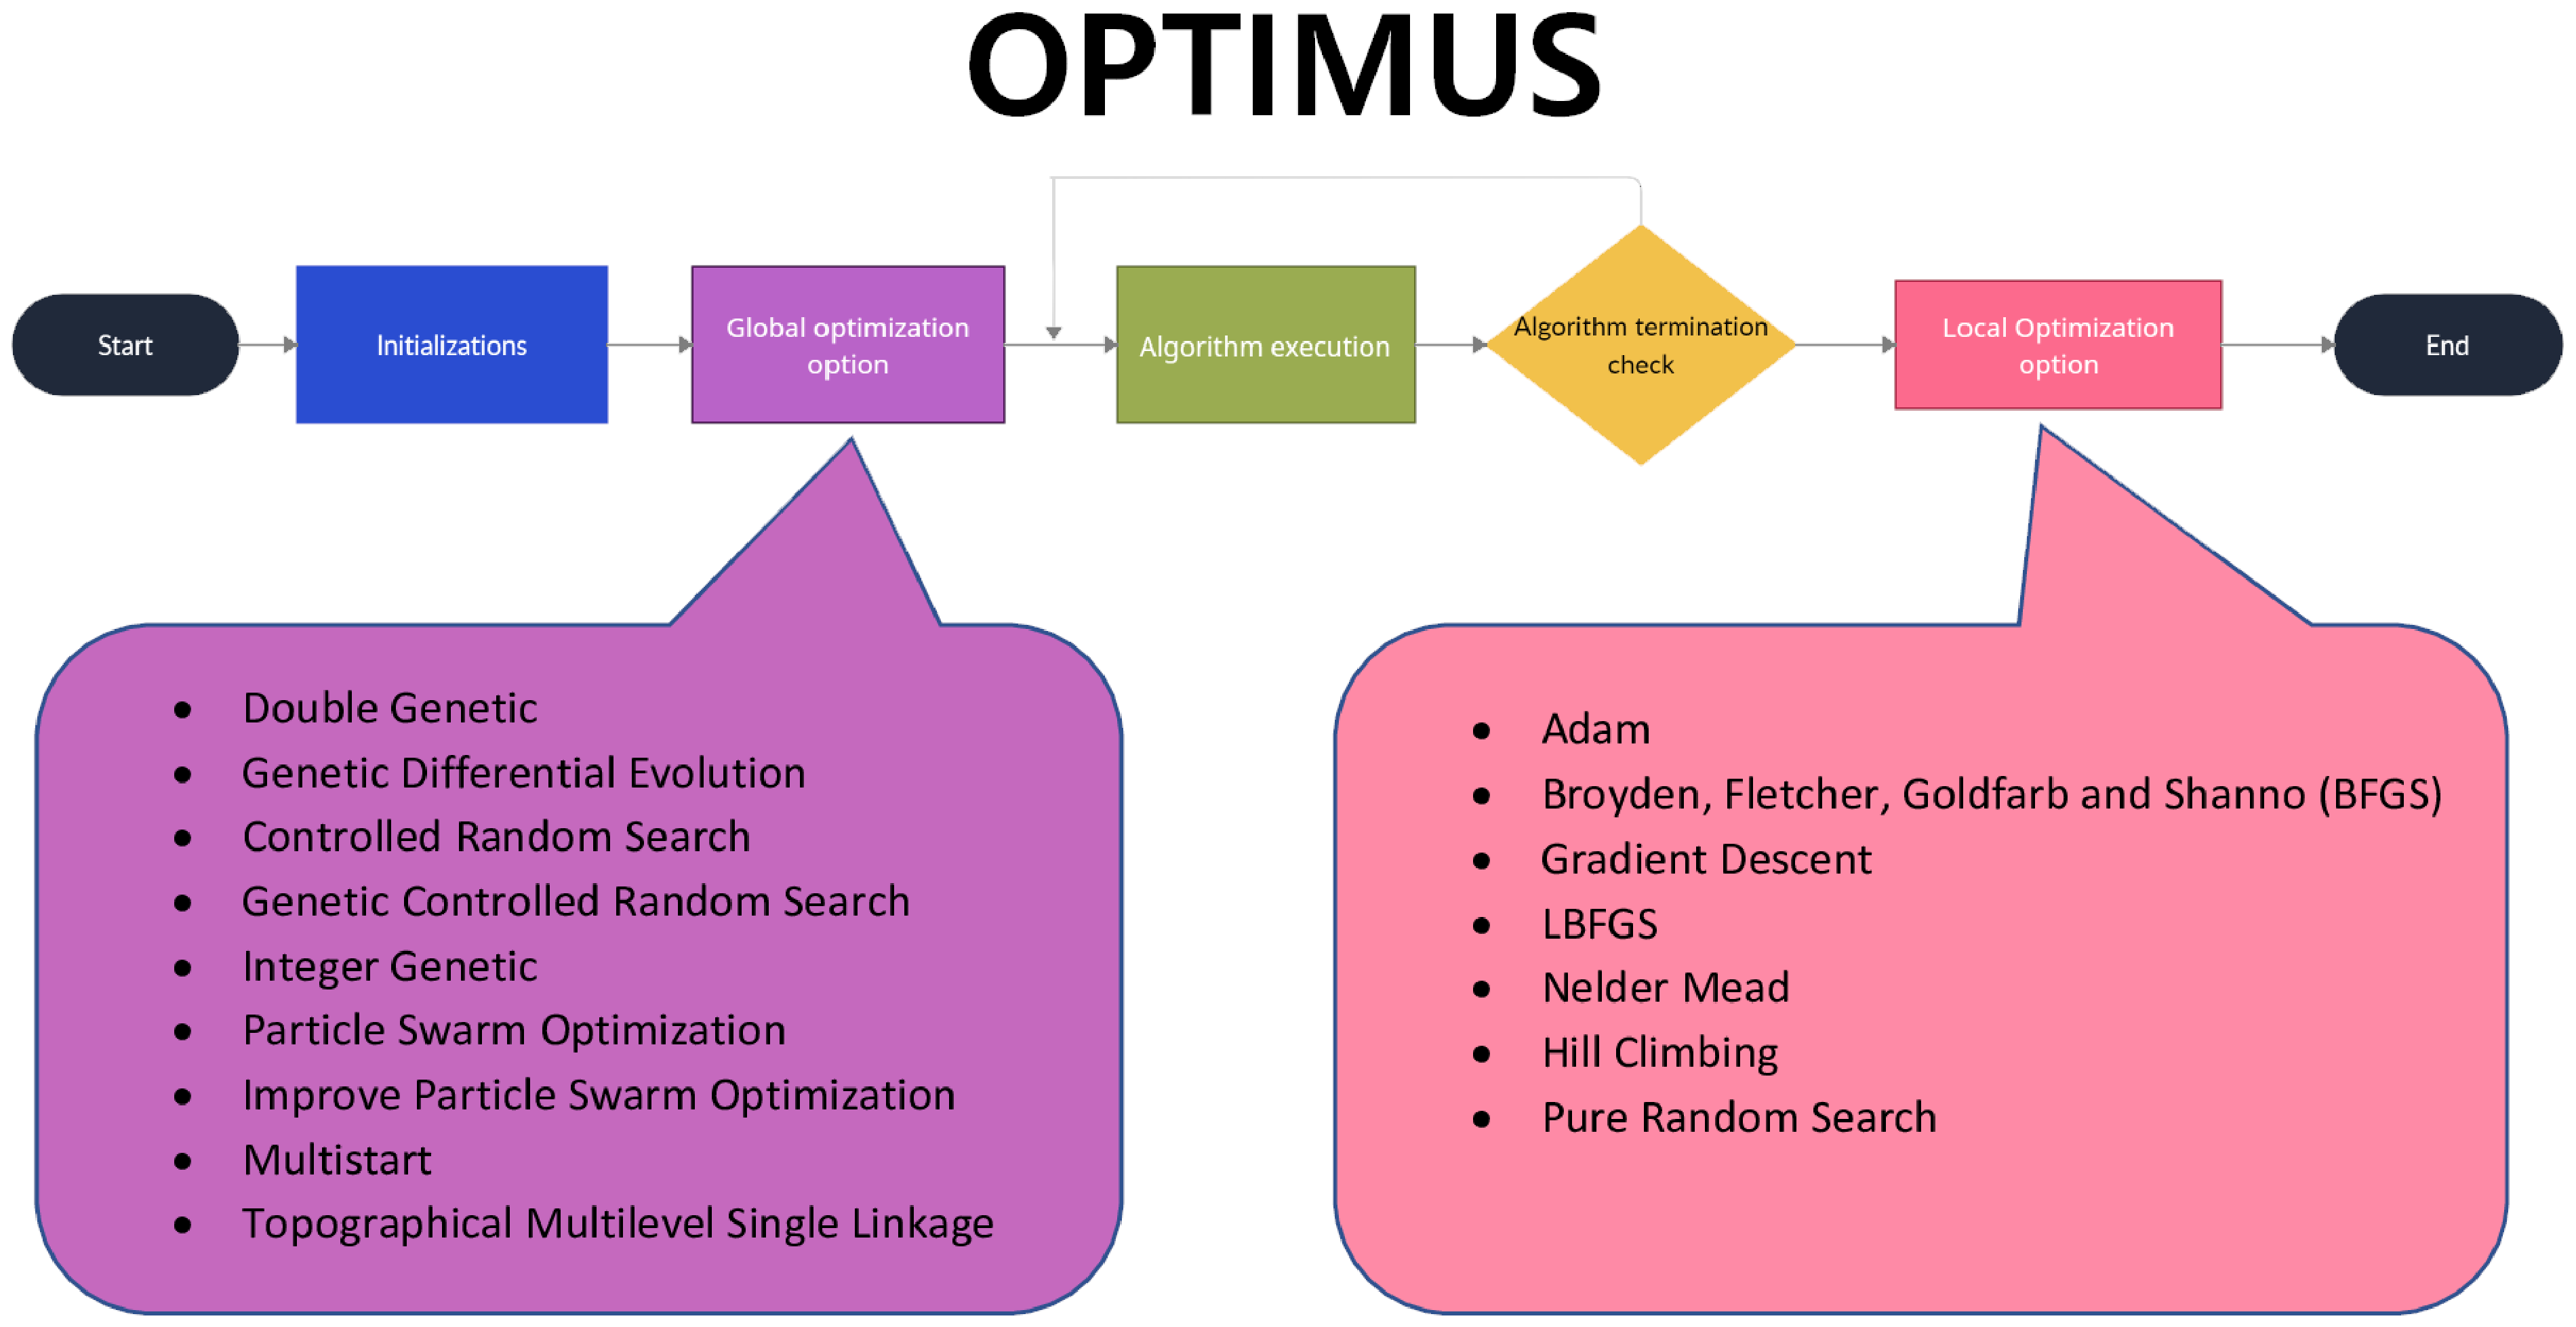
\includegraphics[scale=0.2]{optimus_abstract}

\caption{The steps of a typical optimization process using Optimums.\label{fig:optSteps}}
\end{figure}


\section{Experiments \label{sec:Experiments}}

To assess the ability of the software package to adapt to different
problems, a series of experiments were performed under different conditions.
In the first series of experiments different global optimization techniques
were applied to a series of objective functions that one can locate
in the relevant literature. In the second series of experiments, the
proposed software was applied to a difficult problem from the field
of chemistry, that of finding the minimum potential energy of N interacting
atoms of molecules. In the third set of experiments, the scaling of
the required number of function calls was evaluated for a parallel
technique applied to a difficult problem from the global optimization
space, where the problem dimension was constantly increasing. In the
last set of experiments, different global optimization techniques
were applied to train artificial neural networks. Finally, an additional
set of experiments was executed where some of the implemented global
optimization techniques were applied to a series of constrained optimization
problems.

\subsection{Test functions}

Some of the proposed methods are tested on a series of well - known
test problems from the relevant literature. These problems are used
by many researchers in the field. The description of the test functions
has as follows:
\begin{itemize}
\item \textbf{Griewank2} function. This objective function is defined as:
\[
f(x)=1+\frac{1}{200}\sum_{i=1}^{2}x_{i}^{2}-\prod_{i=1}^{2}\frac{\cos(x_{i})}{\sqrt{(i)}},\quad x\in[-100,100]^{2}
\]
\item \textbf{Rastrigin} function. The function is provided by
\[
f(x)=x_{1}^{2}+x_{2}^{2}-\cos(18x_{1})-\cos(18x_{2}),\quad x\in[-1,1]^{2}
\]
\item \textbf{Shekel 7} function.
\end{itemize}
\[
f(x)=-\sum_{i=1}^{7}\frac{1}{(x-a_{i})(x-a_{i})^{T}+c_{i}}
\]

with $x\in[0,10]^{4}$ and $a=\left(\begin{array}{cccc}
4 & 4 & 4 & 4\\
1 & 1 & 1 & 1\\
8 & 8 & 8 & 8\\
6 & 6 & 6 & 6\\
3 & 7 & 3 & 7\\
2 & 9 & 2 & 9\\
5 & 3 & 5 & 3
\end{array}\right),\ c=\left(\begin{array}{c}
0.1\\
0.2\\
0.2\\
0.4\\
0.4\\
0.6\\
0.3
\end{array}\right)$
\begin{itemize}
\item \textbf{Shekel 5 }function.
\end{itemize}
\[
f(x)=-\sum_{i=1}^{5}\frac{1}{(x-a_{i})(x-a_{i})^{T}+c_{i}}
\]
 

with $x\in[0,10]^{4}$ and $a=\left(\begin{array}{cccc}
4 & 4 & 4 & 4\\
1 & 1 & 1 & 1\\
8 & 8 & 8 & 8\\
6 & 6 & 6 & 6\\
3 & 7 & 3 & 7
\end{array}\right),\ c=\left(\begin{array}{c}
0.1\\
0.2\\
0.2\\
0.4\\
0.4
\end{array}\right)$. 
\begin{itemize}
\item \textbf{Shekel 10} function.
\end{itemize}
\[
f(x)=-\sum_{i=1}^{10}\frac{1}{(x-a_{i})(x-a_{i})^{T}+c_{i}}
\]
 

with $x\in[0,10]^{4}$ and $a=\left(\begin{array}{cccc}
4 & 4 & 4 & 4\\
1 & 1 & 1 & 1\\
8 & 8 & 8 & 8\\
6 & 6 & 6 & 6\\
3 & 7 & 3 & 7\\
2 & 9 & 2 & 9\\
5 & 5 & 3 & 3\\
8 & 1 & 8 & 1\\
6 & 2 & 6 & 2\\
7 & 3.6 & 7 & 3.6
\end{array}\right),\ c=\left(\begin{array}{c}
0.1\\
0.2\\
0.2\\
0.4\\
0.4\\
0.6\\
0.3\\
0.7\\
0.5\\
0.6
\end{array}\right)$
\begin{itemize}
\item \textbf{Test2N} function. This function is given by the equation 
\[
f(x)=\frac{1}{2}\sum_{i=1}^{n}x_{i}^{4}-16x_{i}^{2}+5x_{i},\quad x_{i}\in[-5,5].
\]
This objective function has $2^{n}$ local minima in the specified
range. During the conducted experiments the values $n=4,5,6,7$ were
used.
\end{itemize}
The experiments were performed using the above objective functions
and ran 30 times using a different seed for the random number generator
each time. During the execution of the experiments, the genetic algorithm
(DoubleGenetic method) was used as a global optimizer in two versions:
one without a local optimization method and one with periodic application
of the bfgs method at a rate of 5\% on the chromosomes in every generation.
The execution parameters for the genetic algorithm are listed in Table
\ref{tab:Experimental-settings}. The experimental results for the
two variants of the genetic algorithm are listed in Table \ref{tab:results}.
The numbers in cells denote average function calls for the 30 independent
runs. The numbers in parentheses show the percentage of finding the
global minimum in the 30 runs. If this number is absent, it means
that the algorithm discovered the global minimum in all 30 executions.
In this table, the line SUM represents the sum of the function calls.
The experimental results indicate that the usage of a local search
method in combination with the genetic algorithm significantly reduces
the required number of average function calls and also improves the
reliability of the method in finding the global minimum. Of course,
periodically applying a local minimization method to some of the chromosomes
drastically increases the required execution time, but the large reduction
in the total number of calls required is a big advantage of its application.
\begin{table}
\caption{Experimental settings\label{tab:Experimental-settings}}

\centering{}%
\begin{tabular}{>{\centering}p{0.49\textwidth}>{\centering}p{0.49\textwidth}}
\hline 
\textbf{PARAMETER} & \textbf{VALUE}\tabularnewline
\hline 
CHROMOSOMES & 200\tabularnewline
CROSSOVER RATE & 90\%\tabularnewline
MUTATION RATE & 5\%\tabularnewline
GENERATIONS & 200\tabularnewline
LOCAL SEARCH METHOD & bfgs\tabularnewline
\hline 
\end{tabular}
\end{table}

\begin{table}
\caption{Experimental results for some test functions using a series of global
optimization methods.\label{tab:results}}

\centering{}%
\begin{tabular}{>{\centering}p{0.33\textwidth}>{\centering}p{0.33\textwidth}>{\centering}p{0.33\textwidth}}
\hline 
\textbf{FUNCTION} & \textbf{GENETIC} & \textbf{GENETIC WITH LOCAL}\tabularnewline
\hline 
GRIEWANK2 & 9298(0.97) & 10684\tabularnewline
RASTRIGIN & 8967 & 11038\tabularnewline
SHEKEl5 & 19403(0.70) & 9222\tabularnewline
SHEKEL7 & 16376(0.80) & 8836\tabularnewline
SHEKEL10 & 19829(0.77) & 8729\tabularnewline
TEST2N4 & 17109 & 7786\tabularnewline
TEST2N5 & 19464 & 8264\tabularnewline
TEST2N6 & 24217 & 8868\tabularnewline
TEST2N7 & 26824 & 9376\tabularnewline
\textbf{SUM} & \textbf{161487(0.92)} & \textbf{82803}\tabularnewline
\hline 
\end{tabular}
\end{table}


\subsection{The Lennard Jones potential}

The molecular conformation corresponding to the global minimum of
the energy of N atoms interacting via the Lennard-Jones potential
\cite{Jones,jonesNew} is used as a test case here. The function to
be minimized is given by:
\begin{equation}
V_{LJ}(r)=4\epsilon\left[\left(\frac{\sigma}{r}\right)^{12}-\left(\frac{\sigma}{r}\right)^{6}\right]\label{eq:potential}
\end{equation}
For testing purposes the method \textbf{NeuralMinimizer} of the package
was applied to the above problem for a variety of number of atoms
and the results are shown in Table \ref{tab:potential}. This method
was experimentally compared with two other techniques in the software
package, the method DoubleGenetic and the method Pso. In all cases
the number of chromosomes (or particles) was set to 100 and the maximum
number of allowed iterations was set to 200. As can be seen from the
experimental results, the method NeuralMinimizer requires a significantly
reduced number of function calls compared to the other two, while
its reliability in finding the global minimum for the potential remains
high even when the number of atoms participating in the potential
increases significantly.
\begin{table}[H]
\caption{Optimizing the Potential problem for different number of atoms.\label{tab:potential}}

\centering{}%
\begin{tabular}{>{\centering}p{0.24\textwidth}>{\centering}p{0.24\textwidth}>{\centering}p{0.24\textwidth}>{\centering}p{0.24\textwidth}}
\hline 
\textbf{ATOMS} & \textbf{GENETIC} & \textbf{PSO} & \textbf{NEURALMINIMIZER}\tabularnewline
\hline 
3 & 18902 & 9936 & 1192\tabularnewline
4 & 17806 & 12560 & 1964\tabularnewline
5 & 18477 & 12385 & 2399\tabularnewline
6 & 19069(0.20) & 9683 & 3198\tabularnewline
7 & 16390(0.33) & 10533(0.17) & 3311(0.97)\tabularnewline
8 & 15924(0.50) & 8053(0.50) & 3526\tabularnewline
9 & 15041(0.27) & 9276(0.17) & 4338\tabularnewline
10 & 14817(0.03) & 7548(0.17) & 5517(0.87)\tabularnewline
11 & 13885(0.03) & 6864(0.13) & 6588(0.80)\tabularnewline
12 & 14435(0.17) & 12182(0.07) & 7508(0.83)\tabularnewline
13 & 14457(0.07) & 10748(0.03) & 6717(0.77)\tabularnewline
14 & 13906(0.07) & 14235(0.13) & 6201(0.93)\tabularnewline
15 & 12832(0.10) & 12980(0.10) & 7802(0.90)\tabularnewline
\textbf{AVERAGE} & \textbf{205941(0.37)} & \textbf{137134(0.42)} & \textbf{60258(0.93)}\tabularnewline
\hline 
\end{tabular}
\end{table}


\subsection{Parallel optimization}

The High Conditioned Elliptic function, defined as 
\[
f(x)=\sum_{i=1}^{n}\left(10^{6}\right)^{\frac{i-1}{n-1}}x_{i}^{2}
\]
 is used as a test case to measure the scalability of the parallel
global optimization technique denoted as ParallelDe. This method was
applied to the problem with dimension increasing from 2 to 15 and
for a different number of processing threads. The experimental results
are shown in diagram form in Figure \ref{fig:Scalability}. As one
observes from the figure, the number of calls required to find the
global minimum decreases as the total processing threads increase,
although the problem becomes increasingly difficult with increasing
dimension.

\begin{figure}[H]
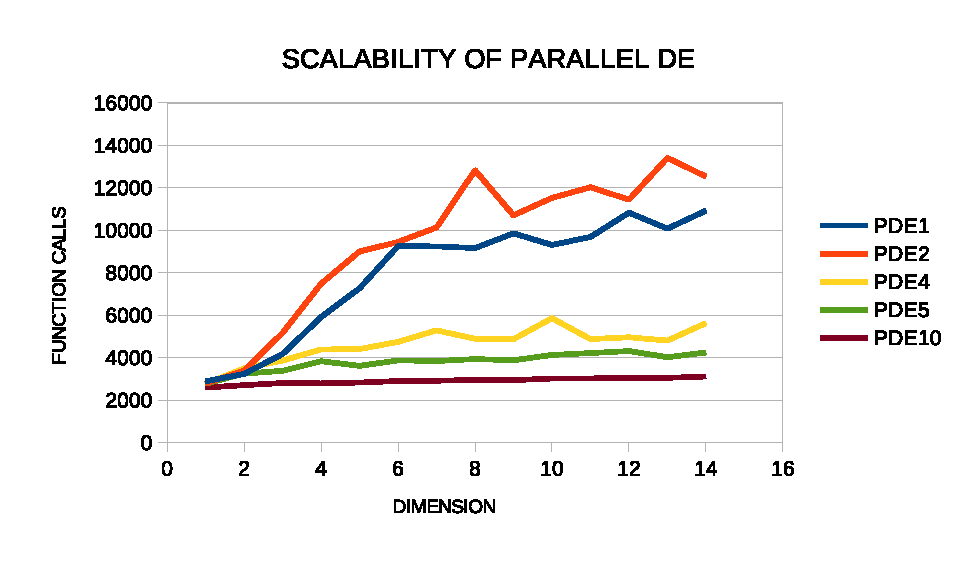
\includegraphics[scale=0.7]{parallelde_scale}

\caption{Scalabilty of the ParallelDe method.\label{fig:Scalability}}
\end{figure}


\subsection{Rbf training}

An RBF network is machine learning model and in function form is defined
as:\textbf{
\begin{equation}
y\left(\overrightarrow{x}\right)=\sum_{i=1}^{k}w_{i}\phi\left(\left\Vert \overrightarrow{x}-\overrightarrow{c_{i}}\right\Vert \right)\label{eq:firstrbf}
\end{equation}
}These models have been used in a wide series of problems, such as
solutions of differential equations \cite{rbfde1,rbfde2}, issues
of communication \cite{rbfnetwork1,rbfnetwork2},\textbf{ }problems
from physics \cite{rbfphysics1,rbfphysics2}, chemistry problems \cite{rbfchemistry1,rbfchemistry2},\textbf{
}economics \cite{rbfecon0,rbfecon1,rbfecon2}, network security \cite{rbf_dos1,rbf_dos2}
etc. The training error RBF networks is defined as: 
\begin{equation}
E(y(x,g))=\sum_{i=1}^{m}\left(y\left(x_{i},g\right)-t_{i}\right)^{2}\label{eq:eqrbf}
\end{equation}
In the previous equation, the constant $m$ stands for the number
of input patterns and the values $t_{i}$ represent the expected output
for the every input vector $x_{i}$. The vector $g$ denotes the parameters
of the RBF network. In most cases, the equation \ref{eq:eqrbf} is
minimized through a two - phase procedure. During the first phase,
a subset of the parameters of the network, called centers and variances,
are calculated using the well - known K-Means algorithm \cite{kmeans}.
During the second phase, a linear system is solved for the calculation
of the weight set $w_{i},\ i=1,..,k$. 

Here, in this series of experiments two methods of the OPTIMUS package,
the genetic algorithm and the particle swarm optimization, was used
to minimize the equation \ref{eq:eqrbf}. The RBF network was applied
on a series of classification problems, described in various papers
\cite{tsoulosAI,tsoulosQFC}. The comparative results are shown in
Table \ref{tab:Experimental-results}. The RBF network was implemented
in ANSI C++ using the freely available Armadillo library \cite{Armadillo}.
The experiments were validated using the 10-fold validation technique.
Furthermore, all the experiments were conducted 30 times. In each
execution a different seed for the random number generator was used.
The average classification error on test set is reported in the table
with the experimental results and the number of weights $k$ was set
to $k=10.$ The table has the following organization:
\begin{enumerate}
\item The column DATASET defines the name of the experimental dataset.
\item The column KRBF stands for classic training method for RBF networks
using the previous mentioned method of two phases.
\item The column GENETIC stands for the application of a genetic algorithm
with 200 chromosomes.
\item The column PESO represents the results for the application of the
particle swarm optimization method with 200 particles.
\item An additional line (with the symbolic name AVERAGE) has been added
at the end of the table, in which the average classification error
for each method is displayed. 
\end{enumerate}
As can be deduced from the experimental results, the global optimization
methods of the proposed software package were applied with great success
to such a difficult and complex problem as that of training a neural
network. Furthermore, both genetic algorithm and particle swarm optimization
significantly outperform the traditional technique in terms of average
test error.

\begin{table}[h]
\caption{Classification error for different datasets.\label{tab:Experimental-results}}

\centering{}%
\begin{tabular}{>{\centering}p{0.24\textwidth}>{\centering}p{0.24\textwidth}>{\centering}p{0.24\textwidth}>{\centering}p{0.24\textwidth}}
\hline 
\textbf{DATASET} & \textbf{KRBF} & \textbf{GENETIC} & \textbf{PESO}\tabularnewline
\hline 
Alcohol & 46.63\% & 25.08\% & 29.23\%\tabularnewline
Appendicitis & 12.23\% & 16.00\% & 14.93\%\tabularnewline
Australian & 34.89\% & 24.53\% & 23.63\%\tabularnewline
Balance & 33.42\% & 14.98\% & 15.08\%\tabularnewline
Dermatology & 62.34\% & 36.41\% & 35.39\%\tabularnewline
Glass & 50.16\% & 49.76\% & 53.83\%\tabularnewline
Hayes Roth & 64.36\% & 37.18\% & 37.87\%\tabularnewline
Heart & 31.20\% & 18.60\% & 17.38\%\tabularnewline
HouseVotes & 6.13\% & 3.77\% & 3.91\%\tabularnewline
Ionosphere & 16.22\% & 10.49\% & 11.96\%\tabularnewline
Liverdisorder & 30.84\% & 28.60\% & 29.25\%\tabularnewline
Mammographic & 21.38\% & 17.34\% & 17.61\%\tabularnewline
Parkinsons & 17.42\% & 16.63\% & 16.91\%\tabularnewline
Pima & 25.78\% & 24.32\% & 23.87\%\tabularnewline
Popfailures & 7.04\% & 5.51\% & 5.84\%\tabularnewline
Saheart & 32.19\% & 29.33\% & 28.80\%\tabularnewline
Sonar & 27.85\% & 20.78\% & 21.42\%\tabularnewline
Spiral & 44.87\% & 17.18\% & 33.67\%\tabularnewline
Tae & 60.07\% & 53.75\% & 52.69\%\tabularnewline
Wdbc & 7.27\% & 5.45\% & 5.11\%\tabularnewline
Wine & 31.41\% & 9.37\% & 8.02\%\tabularnewline
Z\_F\_S & 13.16\% & 3.89\% & 3.74\%\tabularnewline
ZOO & 21.93\% & 9.53\% & 11.10\%\tabularnewline
\textbf{AVERAGE} & \textbf{30.38\%} & \textbf{20.80\%} & \textbf{21.79\%}\tabularnewline
\hline 
\end{tabular}
\end{table}


\subsection{Application to constrained optimization problems}

The methods proposed in this software can be used even in constrained
optimization problems. Typically a constrained optimization problem
can be formulated as:
\begin{eqnarray}
\min_{x} & f(x) & \mbox{subject to}\nonumber \\
 & g_{i}(x)\le0 & \ i=1,\ldots,m\nonumber \\
 & h_{j}(x)=0 & \ j=1,\ldots,p\label{eq:eq1-1}
\end{eqnarray}
where $x_{i}\in\left[a_{i},b_{i}\right],\ i=1,\ldots,n$, and this
problem has many applications in areas such as as physics \cite{ConPhysics},
astronomy \cite{ConAstro}, chemistry \cite{ConChem}, biology \cite{ConBio}
etc. Also, a variety of methods have been proposed for problems of
this category, such as as Lagrange multiplier methods \cite{cons1},
Trust region methods \cite{cons2}, interval methods \cite{cons3},
differential evolution \cite{cons4} etc.\textbf{ }Constrained optimization
problems can be reduced to unconstrained problems through a series
of operations that introduce penalty factors to ensure that the resulting
global minimum obeys the constraints of the original problem. The
steps to produce the reduced unconstrained problem are the following:\\

\begin{enumerate}
\item \textbf{Set} $v_{1}(x)=f(x)$
\item \textbf{Set} $v_{2}(x)=\sum_{i=1}^{p}h_{i}^{2}(x)$
\item \textbf{Calculate }the new quantity $v_{3}(x)$ for the inequality
constraints: 
\begin{equation}
v_{3}(x)=\sum_{i=1}^{m}G_{i}^{2}\left(g_{i}(x)\right)\label{eq:eq5-1}
\end{equation}
The function $G(x)$ has as follows:
\begin{equation}
G(x)=\begin{cases}
0, & x\le0\\
x, & x>0
\end{cases}\label{eq:eq2-1}
\end{equation}
\item \textbf{Transform} the function to $v(x)$ using:
\begin{equation}
v(x)=v_{1}(x)+\lambda v_{2}(x)+\lambda v_{3}(x)\label{eq:fitness}
\end{equation}
where $\lambda>0$ is a penalty factor.
\end{enumerate}
The following test functions were used found in the the relevant literature.
\begin{itemize}
\item \textbf{Levy} function\cite{Levy}. The function is defined as: 
\[
\min_{x}f(x)=-x_{1}-x_{2}
\]
where $x\in[0,1]^{2}$ and the associated constraints are: 
\[
g_{1}(x)=\left\lfloor \left(x_{1}-1\right)^{2}+\left(x_{2}-1\right)\right\rfloor \left(\frac{1}{2a^{2}}-\frac{1}{2b^{2}}\right)+\left(x_{1}-1\right)\left(x_{2}-1\right)\left(\frac{1}{a^{2}}-\frac{1}{b^{2}}\right)-1\ge0
\]
with $a=2,\ b=0.25$. 
\item \textbf{Salkin} function\cite{Salkin}. The objective function is
defined as: 
\[
\max_{x}f(x)=3x_{1}+x_{2}+2x_{3}+x_{4}-x_{5}
\]
with $1\le x_{1}\le4,\ 80\le x_{2}\le88,\ 30\le x_{3}\le35,\ 145\le x_{4}\le150,\ 0\le x_{5}\le2$
subject to 
\begin{eqnarray*}
g_{1}(x) & = & 25x_{1}-40x_{2}+16x_{3}+21x_{4}+x5\le300\\
g_{2}(x) & = & x_{1}+20x_{2}-50x_{3}+x_{4}-x_{5}\le200\\
g_{3}(x) & = & 60x_{1}+x_{2}-x_{3}+2x_{4}+x_{5}\le600\\
g_{4}(x) & = & -7x_{1}+4x_{2}+15x_{3}-x_{4}+65x_{5}\le700
\end{eqnarray*}
\item \textbf{Hess} function\cite{Hess}. The function is defined as:
\[
\max_{x}f(x)=25\left(x_{1}-2\right)^{2}+\left(x_{2}-2\right)^{2}+\left(x_{3}-1\right)^{2}+\left(x_{4}-4\right)^{2}+\left(x_{5}-1\right)^{2}+\left(x_{6}-4\right)^{2}
\]
with $0\le x_{1}\le5,\ 0\le x_{2}\le1,\ 1\le x_{3}\le5,\ 0\le x_{4}\le6,\ 0\le x_{5}\le5,\ 0\le x_{6}\le10$
subject to:
\begin{eqnarray*}
g_{1}(x) & = & x_{1}+x_{2}-2\ge0\\
g_{2}(x) & = & -x_{1}+x_{2}+6\ge0\\
g_{3}(x) & = & x_{1}-x_{2}+2\ge0\\
g_{4}(x) & = & -x_{1}+3x_{2}+2\ge0\\
g_{5}(x) & = & \left(x_{3}-3\right)^{2}+x_{4}-4\ge0\\
g_{6}(x) & = & \left(x_{5}-3\right)^{2}+x_{6}-4\ge0
\end{eqnarray*}
\item \textbf{Chootinan1} function\cite{choot}. The objective problem is
defined as:
\[
\min_{x}f(x)=5\sum_{i=1}^{4}x_{i}-5\sum_{i=1}^{4}x_{i}^{2}-\sum_{i=1}^{13}x_{i}
\]
with $0\le x_{i}\le1$ for $i=1,..,9,13$, $0\le x_{i}\le100$ for
$i=10,11,12$ subject to:
\begin{eqnarray*}
g_{1}(x) & = & 10-\left(2x_{1}+2x_{2}+x_{10}+x_{11}\right)\ge0\\
g_{2}(x) & = & 10-\left(2x_{1}+2x_{3}+x_{10}+x_{12}\right)\ge0\\
g_{3}(x) & = & 10-\left(2x_{2}+2x_{3}+x_{11}+x_{12}\right)\ge0\\
g_{4}(x) & = & 8x_{1}-x_{10}\ge0\\
g_{5}(x) & = & 8x_{2}-x_{11}\ge0\\
g_{6}(x) & = & 8x_{3}-x_{12}\ge0\\
g_{7}(x) & = & 2x_{4}+x_{5}-x_{10}\ge0\\
g_{8}(x) & = & 2x_{6}+x_{7}-x_{11}\ge0\\
g_{9}(x) & = & 2x_{8}+x_{9}-x_{12}\ge0
\end{eqnarray*}
\item \textbf{G15} function\cite{G15}. The function is defined as:
\[
\min_{x}f(x)=1000-x_{1}^{2}-2x_{2}^{2}-x_{3}^{2}-x_{1}x_{2}-x_{1}x_{3}
\]
where $x\in[0,10]^{3}$ and the associated constraints are:
\begin{eqnarray*}
h_{1}(x) & = & x_{1}^{2}+x_{2}^{2}+x_{3}^{2}-25=0\\
h_{2}(x) & = & 8x_{1}+14x_{2}+7x_{3}-56=0
\end{eqnarray*}
\end{itemize}
Four global optimization methods implemented in the current software
were applied to the previous problems and the average function calls
for 30 independent runs are shown in Table \ref{tabCons}. Once again,
techniques proposed here (NeuralMinimizer and the Improved Pso) have
a significantly lower number of function calls than other established
techniques in global optimization.

\begin{table}
\caption{Average function calls for a variety of optimization methods when
applied to some Constrained Optimization problems.\label{tabCons}}

\centering{}%
\begin{tabular}{>{\centering}p{0.19\linewidth}>{\centering}p{0.19\linewidth}>{\centering}p{0.19\linewidth}>{\centering}p{0.19\linewidth}>{\centering}p{0.19\linewidth}}
\hline 
FUNCTION & NEURALMINIMIZER & Pso & Genetic & IPSO\tabularnewline
\hline 
Levy & 1339 & 6901 & 14872 & 4322\tabularnewline
Salkin & 4230 & 7990 & 20111 & 4970\tabularnewline
Hess & 3653 & 18137 & 20138 & 5344\tabularnewline
Chootinan1 & 7680 & 18794 & 20238 & 6610\tabularnewline
G15 & 22476 & 13498 & 20169 & 12253\tabularnewline
\textbf{Average} & \textbf{7875.6} & \textbf{13064.0} & \textbf{19105.6} & \textbf{6699.8}\tabularnewline
\hline 
\end{tabular}
\end{table}


\section{Conclusions\label{sec:Conclusions}}

In this work, an environment for executing global optimization problems
was presented. In this environment, the user can code the objective
problem using some predefined functions and then has the possibility
to choose one among several global optimization methods to solve the
mentioned problem. In addition, it is given the possibility to choose
to use some local optimization method to enhance the reliability of
the produced results. This programming environment is freely available
and easy to extend to accommodate more global optimization techniques.
It is subject to continuous improvements and some of those planned
for the near future are:
\begin{enumerate}
\item Possibility to port the Optimums tool to other operating systems such
as FreeBSD, Windows etc.
\item Use of modern parallel techniques to speed up the generated results
and implementation of efficient termination techniques. At the present
time, the ParallelDe has been implemented using parallel techniques
and it is expected that parallel implementations will be created for
other global minimization techniques as well. In addition, new termination
techniques specifically designed for parallel techniques should be
devised and implemented.
\item Implementing a GUI interface to control the optimization process.
\item Ability to code the objective function in other programming languages
such as Python, Ada, Fortran etc.
\item Creating a scripting language to efficiently guide the optimization
of objective functions.
\end{enumerate}
\begin{thebibliography}{100}
\bibitem{globalecon1}Zwe-Lee Gaing, Particle swarm optimization to
solving the economic dispatch considering the generator constraints,
IEEE Transactions on \textbf{18} Power Systems, pp. 1187-1195, 2003.

\bibitem{globalecon2}C. D. Maranas, I. P. Androulakis, C. A. Floudas,
A. J. Berger, J. M. Mulvey, Solving long-term financial planning problems
via global optimization, Journal of Economic Dynamics and Control
\textbf{21}, pp. 1405-1425, 1997.

\bibitem{global_physics1}Q. Duan, S. Sorooshian, V. Gupta, Effective
and efficient global optimization for conceptual rainfall-runoff models,
Water Resources Research \textbf{28}, pp. 1015-1031 , 1992.

\bibitem{global_physics2}P. Charbonneau, Genetic Algorithms in Astronomy
and Astrophysics, Astrophysical Journal Supplement \textbf{101}, p.
309, 1995

\bibitem{global_chemistry1}A. Liwo, J. Lee, D.R. Ripoll, J. Pillardy,
H. A. Scheraga, Protein structure prediction by global optimization
of a potential energy function, Biophysics \textbf{96}, pp. 5482-5485,
1999.

\bibitem{global_chemistry2}P.M. Pardalos, D. Shalloway, G. Xue, Optimization
methods for computing global minima of nonconvex potential energy
functions, Journal of Global Optimization \textbf{4}, pp. 117-133,
1994.

\bibitem{global_med1}Eva K. Lee, Large-Scale Optimization-Based Classification
Models in Medicine and Biology, Annals of Biomedical Engineering \textbf{35},
pp 1095-1109, 2007.

\bibitem{global_med2}Y. Cherruault, Global optimization in biology
and medicine, Mathematical and Computer Modelling \textbf{20}, pp.
119-132, 1994.

\bibitem{global_job1}Y. Gao, H. Rong, J.Z. Huang, Adaptive grid job
scheduling with genetic algorithms, Future Generation Computer Systems
\textbf{21}, pp. 151-161, 2005.

\bibitem{global_job2}D.Y. Sha, H.H. Lin, A multi-objective PESO for
job-shop scheduling problems, Expert Systems with Applications \textbf{37},
pp. 1065-1070, 2010.

\bibitem{global_water1}X. Cai, D.C. McKinney, L.S. Lasdon, Solving
nonlinear water management models using a combined genetic algorithm
and linear programming approach, Advances in Water Resources \textbf{24},
pp. 667-676, 2001.

\bibitem{global_water2}S.G. Gino Sophia, V. Ceronmani Sharmila, S.
Suchitra et al, Water management using genetic algorithm-based machine
learning, Soft Comput \textbf{24}, pp. 17153--17165, 2020.

\bibitem{global_network1}Z. Bankovic, D. Stepanovic, S. Bojanic,
O. Nieto - Taladriz, Improving network security using genetic algorithm
approach, Computers \& Electrical Engineering \textbf{33}, pp. 438-451,
2007.

\bibitem{global_network2}S. Paul, I. Dutt, S.N. Choudhri, Design
and implementation of network security using genetic algorithm. Int
J Res Eng Technol \textbf{2}, pp. 172-177, 2013.

\bibitem{global_robot1}A. Tuncer, M. Yildrim, Dynamic path planning
of mobile robots with improved genetic algorithm, Computers \& Electrical
Engineering \textbf{38}, pp. 1564-1572, 2012.

\bibitem{global_robot2}N. Kherici, Y.M. Ben Ali, Using PESO for a
walk of a biped robot, Journal of Computational Science \textbf{5},
pp. 743-749, 2014.

\bibitem{go_symmetry0}B. Freisleben and P. Merz, A genetic local
search algorithm for solving symmetric and asymmetric traveling salesman
problems, In: Proceedings of IEEE International Conference on Evolutionary
Computation, pp. 616-621, 1996.

\bibitem{go_symmetry1}R. Grbi\'{c}, E.K. Nyarko and R. Scitovski,
A modification of the DIRECT method for Lipschitz global optimization
for a symmetric function, J Glob Optim \textbf{57}, pp. 1193--1212,
2013.

\bibitem{go_symmetry2}R. Scitovski, A new global optimization method
for a symmetric Lipschitz continuous function and the application
to searching for a globally optimal partition of a one-dimensional
set, J Glob Optim \textbf{68}, pp. 713--727, 2017.

\bibitem{global_nonlinear1}Barbara Kaltenbacher and William Rundell,
The inverse problem of reconstructing reaction--diffusion systems,
Invese Problems \textbf{36}, 2020.

\bibitem{global_nonlinear2}N. Levashova, A. Gorbachev, R. Argun,
D. Lukyanenko, The Problem of the Non-Uniqueness of the Solution to
the Inverse Problem of Recovering the Symmetric States of a Bistable
Medium with Data on the Position of an Autowave Front., Symmetry \textbf{13},
2021.

\bibitem{global_nonlinear3}Larisa Beilina, Michael V. Klibanov, A
Globally Convergent Numerical Method for a Coefficient Inverse Problem,
SIAM Journal on Scientific Computing \textbf{31},pp. 478-509, 2008. 

\bibitem{go_adaptive1}M. Brunato, R. Battiti, RASH: A Self-adaptive
Random Search Method. In: Cotta, C., Sevaux, M., S�rensen, K. (eds)
Adaptive and Multilevel Metaheuristics. Studies in Computational Intelligence,
vol 136. Springer, Berlin, Heidelberg, 2008.

\bibitem{go_adaptive2}S. Andrad�ttir, A.A. Prudius, A.A., Adaptive
random search for continuous simulation optimization. Naval Research
Logistics \textbf{57}, pp. 583-604, 2010.

\bibitem{go_crs1}W.L. Price, Global optimization by controlled random
search, J Optim Theory Appl \textbf{40}, pp. 333--348, 1983.

\bibitem{go_crs2}P. Kaelo, M.M. Ali, Some Variants of the Controlled
Random Search Algorithm for Global Optimization. J Optim Theory Appl
\textbf{130}, pp. 253--264 (2006).

\bibitem{go_sa1}S. Kirkpatrick, C.D. Gelatt, M.P. Vecchi, Optimization
by simulated annealing, Science \textbf{220}, pp. 671-680, 1983.

\bibitem{go_sa2}K.M.El-Naggar, M.R. AlRashidi, M.F. AlHajri, A.K.
Al-Othman, Simulated Annealing algorithm for photovoltaic parameters
identification, Solar Energy \textbf{86}, pp. 266-274, 2012.

\bibitem{go_sa3}L.M. Rasdi Rere, M.I. Fanany, A.M. Arymurthy, Simulated
Annealing Algorithm for Deep Learning, Procedia Computer Science \textbf{72},
pp. 137-144, 2015.

\bibitem{go_ga1}J. Mc Call, Genetic algorithms for modelling and
optimisation, Journal of Computational and Applied Mathematics \textbf{184},
pp. 205-222, 2005.

\bibitem{go_ga2}C.K.H. Lee, A review of applications of genetic algorithms
in operations management, Elsevier Engineering Applications of Artificial
Intelligence \textbf{76}, pp. 1-12, 2018.

\bibitem{go_ant1}B. Chandra Mohan, R. Baskaran, A survey: Ant Colony
Optimization based recent research and implementation on several engineering
domain, Expert Systems with Applications \textbf{39}, pp. 4618-4627,
2012.

\bibitem{go_ant2}T. Liao, T. St�tzle, M.A. Montes de Oca, M. Dorigo,
A unified ant colony optimization algorithm for continuous optimization,
European Journal of Operational Research \textbf{234}, pp. 597-609,
2014.

\bibitem{go_pso1}D. Wang, D. Tan, L. Liu, Particle swarm optimization
algorithm: an overview. Soft Comput \textbf{22}, pp. 387--408, 2018.

\bibitem{go_pso2}N.K. Jain, U. Nangia, J. Jain, A Review of Particle
Swarm Optimization. J. Inst. Eng. India Ser. B \textbf{99}, pp. 407--411,
2018.

\bibitem{go_pso_genetic_hybrid1}D.H. Kim, A. Abraham, J.H. Cho, A
hybrid genetic algorithm and bacterial foraging approach for global
optimization, Information Sciences \textbf{177}, pp. 3918-3937, 2007.

\bibitem{go_pso_genetic_hybrid2}Y.T. Kao, E. Zahara, A hybrid genetic
algorithm and particle swarm optimization for multimodal functions,
Applied Soft Computing \textbf{8}, pp. 849-857, 2008.

\bibitem{ga_fuzzy}G.T. Reddy, M.P.K. Reddy, K. Lakshmanna et al,
Hybrid genetic algorithm and a fuzzy logic classifier for heart disease
diagnosis, Evol. Intel. \textbf{13}, pp. 185--196, 2020.

\bibitem{ga_kmeans}M.D. Anisur Rahman, M.D. Zahidul Islam, A hybrid
clustering technique combining a novel genetic algorithm with K-Means,
Knowledge-Based Systems \textbf{71}, pp. 345-365, 2014.

\bibitem{pso_aco1}T. Niknam, An efficient hybrid evolutionary algorithm
based on PESO and ACO for distribution feeder reconfiguration, European
Transactions on Electrical Power \textbf{20}, pp. 575-590, 2010.

\bibitem{pso_aco2}M.K. Patel, M.R. Kabat, C.R. Tripathy, A hybrid
ACO/PESO based algorithm for QoS multicast routing problem, Ain Shams
Engineering Journal \textbf{5}, pp. 113-120, 2014.

\bibitem{pso_aco3}A.K. Dubey, A. Kumar, R. Agrawal, An efficient
ACO-PSO-based framework for data classification and preprocessing
in big data, Evol. Intel. \textbf{14}, pp. 909--922, 2021.

\bibitem{hybrid1}Offord C., Bajzer �. (2001) A Hybrid Global Optimization
Algorithm Involving Simplex and Inductive Search. In: Alexandrov V.N.,
Dongarra J.J., Juliano B.A., Renner R.S., Tan C.J.K. (eds) Computational
Science - ICCS 2001. ICCS 2001. Lecture Notes in Computer Science,
vol 2074. Springer, Berlin, Heidelberg.

\bibitem{go_local1}S. Li, M. Tan, I. W. Tsang, J. T. -Y. Kwok, A
Hybrid PSO-BFGS Strategy for Global Optimization of Multimodal Functions,
IEEE Transactions on Systems, Man, and Cybernetics, Part B (Cybernetics)
\textbf{41}, pp. 1003-1014, 2011.

\bibitem{go_local2}H. Badem, A. Basturk, A. Caliskan, M.E. Yuksel,
A new hybrid optimization method combining artificial bee colony and
limited-memory BFGS algorithms for efficient numerical optimization,
Applied Soft Computing \textbf{70}, pp. 826-844, 2018.

\bibitem{go_local3}A.A. Nagra, F. Han, Q.H. Ling, An improved hybrid
self-inertia weight adaptive particle swarm optimization algorithm
with local search, Engineering Optimization \textbf{51}, pp. 1115-1132,
2018.

\bibitem{genetic_physics1}S.Q. Wu, M. Ji, C.Z. Wang, M.C. Nguyen,
X. Zhao, K. Umemoto, R. M. Wentzcovitch, K. M. Ho, An adaptive genetic
algorithm for crystal structure prediction, Journal of Physics: Condensed
Matter \textbf{26}, 035402, 2013.

\bibitem{genetic_physics2}M. Honda, Application of genetic algorithms
to modelings of fusion plasma physics, Computer Physics Communications
\textbf{231}, pp. 94-106, 2018.

\bibitem{genetic_physics3}X.L. Luo, J. Feng, H.H. Zhang, A genetic
algorithm for astroparticle physics studies, Computer Physics Communications
\textbf{250}, 106818, 2020.

\bibitem{pso_physics1}M. Ye, X. Wang, Y. Xu, Parameter extraction
of solar cells using particle swarm optimization, Journal of Applied
Physics \textbf{105}, 094502. 2009.

\bibitem{pso_physics2}A. Belkadi, L. Ciarletta, D. Theilliol, Particle
swarm optimization method for the control of a fleet of Unmanned Aerial
Vehicles, Journal of Physics: Conference Series, Volume 659, 12th
European Workshop on Advanced Control and Diagnosis (ACD 2015) 19--20
November 2015, Pilsen, Czech Republic.

\bibitem{async1}M. Depolli, R. Trobec, B. Filipi\v{c}, Asynchronous
Master-Slave Parallelization of Differential Evolution for Multi-Objective
Optimization, Evolutionary Computation \textbf{21}, pp. 261-291, 2013.

\bibitem{async2}A. P. Engelbrecht, Asynchronous particle swarm optimization
with discrete crossover, In: 2014 IEEE Symposium on Swarm Intelligence,
Orlando, FL, USA, 2014, pp. 1-8.

\bibitem{async3}F. Bourennani, Cooperative asynchronous parallel
particle swarm optimization for large dimensional problems, International
Journal of Applied Metaheuristic Computing (IJAMC) \textbf{10.3},
pp. 19-38, 2019.

\bibitem{parallel-multistart}J. Larson and S.M. Wild, Asynchronously
parallel optimization solver for finding multiple minima, Mathematical
Programming Computation \textbf{10}, pp. 303-332, 2018.

\bibitem{parallel-multistart2}H.P.J. Bolton, J.F. Schutte, A.A. Groenwold,
Multiple Parallel Local Searches in Global Optimization. In: Dongarra
J., Kacsuk P., Podhorszki N. (eds) Recent Advances in Parallel Virtual
Machine and Message Passing Interface. EuroPVM/MPI 2000. Lecture Notes
in Computer Science, vol 1908. Springer, Berlin, Heidelberg, 2000.

\bibitem{gpu1}Y. Zhou and Y. Tan, GPU-based parallel particle swarm
optimization, In: 2009 IEEE Congress on Evolutionary Computation,
2009, pp. 1493-1500.

\bibitem{gpu2}L. Dawson and I. Stewart, Improving Ant Colony Optimization
performance on the GPU using CUDA, In: 2013 IEEE Congress on Evolutionary
Computation, 2013, pp. 1901-1908.

\bibitem{gpu3}Barkalov, K., Gergel, V. Parallel global optimization
on GPU. J Glob Optim \textbf{66}, pp. 3--20, 2016.

\bibitem{baron}N.V. Sahinidis, BARON: A general purpose global optimization
software package, J Glob Optim \textbf{8}, pp. 201--205, 1996.

\bibitem{merlin}D.G. Papageorgiou, I.N. Demetropoulos, I.E. Lagaris,
Computer Physics Communications \textbf{159}, pp. 70-71, 2004.

\bibitem{deoptim}K. Mullen, D. Ardia, D.L. Gil, D. Windover, J. Cline,
DEoptim: An R Package for Global Optimization by Differential Evolution,
Journal of Statistical Software \textbf{40}, pp. 1-26, 2011.

\bibitem{pdoublepop}I.G. Tsoulos, A. Tzallas, D. Tsalikakis, PDoublePop:
An implementation of parallel genetic algorithm for function optimization,
Computer Physics Communications \textbf{209}, pp. 183-189, 2016.

\bibitem{paradiseo}J. Dreo, A. Liefooghe, S. Verel, M. Schoenauer,
J.J. Merelo, A. Quemy, B. Bouvier, J. Gmys, Paradiseo: from a modular
framework for evolutionary computation to the automated design of
metaheuristics ---22 years of Paradiseo---, GECCO'21: Proceedings
of the Genetic and Evolutionary Computation Conference Companion,
1522--1530, 2021.

\bibitem{pagmo}F. Biscani, D. Izzo, A parallel global multiobjective
framework for optimization: pagmo, Journal of Open Source Software
\textbf{5}, 2338, 2020.

\bibitem{de_main_paper}R. Storn, On the usage of differential evolution
for function optimization, In: Proceedings of North American Fuzzy
Information Processing, pp. 519-523, 1996.

\bibitem{de_datamining}I. Triguero, S. Garcia, F. Herrera, Differential
evolution for optimizing the positioning of prototypes in nearest
neighbor classification, Pattern Recognition \textbf{44}, pp. 901-916,
2011.

\bibitem{de_symmetry1}Y.H. Li, J.Q. Wang, X.J. Wang, Y.L. Zhao, X.H.
Lu, D.L. Liu, Community Detection Based on Differential Evolution
Using Social Spider Optimization, Symmetry \textbf{9}, 2017.

\bibitem{de_symmetry3}W. Yang, E.M. Dilanga Siriwardane, R. Dong,
Y. Li, J. Hu, Crystal structure prediction of materials with high
symmetry using differential evolution, J. Phys.: Condens. Matter \textbf{33}
455902, 2021.

\bibitem{de_symmetry6}C.Y. Lee, C.H. Hung, Feature Ranking and Differential
Evolution for Feature Selection in Brushless DC Motor Fault Diagnosis
, Symmetry \textbf{13}, 2021.

\bibitem{de_symmetry7}S. Saha, R. Das, Exploring differential evolution
and particle swarm optimization to develop some symmetry-based automatic
clustering techniques: application to gene clustering, Neural Comput
\& Applic \textbf{30}, pp. 735--757, 2018.

\bibitem{gende}V. Charilogis, I.G. Tsoulos, A. Tzallas, E. Karvounis,
Modifications for the Differential Evolution Algorithm, Symmetry \textbf{14},
447, 2022. 

\bibitem{parallelDe}V. Charilogis, I.G. Tsoulos, A Parallel Implementation
of the Differential Evolution Method, Analytics \textbf{2}, pp. 17-30,
2023.

\bibitem{openMp}R. Chandra, L. Dagum, D. Kohr, D. Maydan,J. McDonald
and R. Menon, Parallel Programming in OpenMP, Morgan Kaufmann Publishers
Inc., 2001.

\bibitem{doublepop_tsoulos}I.G. Tsoulos, Modifications of real code
genetic algorithm for global optimization, Applied Mathematics and
Computation \textbf{203}, pp. 598-607, 2008.

\bibitem{genetic1}J.F.Gon�alves, J.J.M. Mendes, M.G.C. Resende, A
genetic algorithm for the resource constrained multi-project scheduling
problem, European Journal of Operational Research \textbf{189}, pp.
1171-1190, 2008.

\bibitem{genetic2}W.Ho, G.T.S. Ho, P. Ji, H.C.W. Lau, A hybrid genetic
algorithm for the multi-depot vehicle routing problem, Engineering
Applications of Artificial Intelligence \textbf{21}, pp. 548-557,
2008.

\bibitem{genetic3}J.F. Gon�alves, M.G.C. Resende, Biased random-key
genetic algorithms for combinatorial optimization. J Heuristics \textbf{17},
pp. 487--525, 2011.

\bibitem{genetic4}M. Turrin, P. Buelow, R. Stouffs, Design explorations
of performance driven geometry in architectural design using parametric
modeling and genetic algorithms, Advanced Engineering Informatics
\textbf{25}, pp. 656-675, 2011.

\bibitem{tsp1}J. Kaabi, Y. Harrath, Permutation rules and genetic
algorithm to solve the traveling salesman problem, Arab Journal of
Basic and Applied Sciences \textbf{26}, pp. 283-291, 2019.

\bibitem{tsp2}Q.M. Ha, Y. Deville, Q.D. Pham et al., A hybrid genetic
algorithm for the traveling salesman problem with drone, J Heuristics
\textbf{26}, pp. 219--247, 2020.

\bibitem{pathPlanning}F. Ahmed, K. Deb, Multi-objective optimal path
planning using elitist non-dominated sorting genetic algorithms, Soft
Comput \textbf{17}, pp. 1283--1299, 2013.

\bibitem{ge}M. O'Neill, C. Ryan, Grammatical Evolution, IEEE Trans.
Evolutionary Computation \textbf{5}, pp. 349-358, 2001.

\bibitem{gcrs}V. Charilogis, I.G. Tsoulos, A. Tzallas, N. Anastasopoulos,
An Improved Controlled Random Search Method, Symmetry \textbf{13},
1981, 2021. 

\bibitem{psoApp1}M. Ye, X. Wang, Y. Xu, Parameter extraction of solar
cells using particle swarm optimization, Journal of Applied Physics
\textbf{105}, 094502, 2009.

\bibitem{psoApp2}Y. Wang, J. Lv, L. Zhu, Y. Ma, Crystal structure
prediction via particle-swarm optimization, Phys. Rev. B \textbf{82},
094116, 2010.

\bibitem{psoApp3}M. Weiel, M. G�tz, A. Klein et al, Dynamic particle
swarm optimization of biomolecular simulation parameters with flexible
objective functions. Nat Mach Intell \textbf{3}, pp. 727--734, 2021.

\bibitem{ipso}V. Charilogis, I.G. Tsoulos, Toward an Ideal Particle
Swarm Optimizer for Multidimensional Functions, Information \textbf{13},
217, 2022.

\bibitem{multistart-tsp}Li W., A Parallel Multi-start Search Algorithm
for Dynamic Traveling Salesman Problem. In: Pardalos P.M., Rebennack
S. (eds) Experimental Algorithms. SEA 2011. Lecture Notes in Computer
Science, vol 6630. Springer, Berlin, Heidelberg, 2011.

\bibitem{multistart-vehicle}Olli Br�ysy, Geir Hasle, Wout Dullaert,
A multi-start local search algorithm for the vehicle routing problem
with time windows, European Journal of Operational Research \textbf{159},
pp. 586-605, 2004.

\bibitem{multistart_fac}Mauricio G.C. Resende, Renato F. Werneck,A
hybrid multistart heuristic for the uncapacitated facility location
problem, European Journal of Operational Research \textbf{174}, pp.
54-68, 2006.

\bibitem{multistart_clique}E. Marchiori, Genetic, Iterated and Multistart
Local Search for the Maximum Clique Problem. In: Cagnoni S., Gottlieb
J., Hart E., Middendorf M., Raidl G.R. (eds) Applications of Evolutionary
Computing. EvoWorkshops 2002. Lecture Notes in Computer Science, vol
2279. Springer, Berlin, Heidelberg. 

\bibitem{multistart_fire}Gomes M.I., Afonso L.B., Chibeles-Martins
N., Fradinho J.M. (2018) Multi-start Local Search Procedure for the
Maximum Fire Risk Insured Capital Problem. In: Lee J., Rinaldi G.,
Mahjoub A. (eds) Combinatorial Optimization. ISCO 2018. Lecture Notes
in Computer Science, vol 10856. Springer, Cham. https://doi.org/10.1007/978-3-319-96151-4\_19

\bibitem{multistart-aero}Streuber, Gregg M. and Zingg, David. W.,
Evaluating the Risk of Local Optima in Aerodynamic Shape Optimization,
AIAA Journal 59, pp. 75-87, 2012.

\bibitem{tmlsl}M.M. Ali, C. Storey, Topographical multilevel single
linkage, J. Global Optimization \textbf{5}, pp. 349--358,1994

\bibitem{mincenter}V. Charilogis, I.G. Tsoulos, MinCentre: using
clustering in global optimisation, International Journal of Computational
Intelligence Studies \textbf{11}, pp. 24-35, 2022.

\bibitem{rbf_main1}J. Park, I.W. Sandberg, Approximation and Radial-Basis-Function
Networks, Neural Computation \textbf{5}, pp. 305-316, 1993.

\bibitem{neuralMinimizer}I.G. Tsoulos, A. Tzallas, E. Karvounis,
D. Tsalikakis, NeuralMinimizer, a novel method for global optimization
that incorporates machine learning, Information \textbf{14}, 2, 2023.

\bibitem{powell}M.J.D Powell, A Tolerant Algorithm for Linearly Constrained
Optimization Calculations, Mathematical Programming \textbf{45}, pp.
547-566, 1989. 

\bibitem{lbfgs}D.C. Liu, J. Nocedal, On the Limited Memory Method
for Large Scale Optimization, Mathematical Programming B \textbf{45},
pp. 503-528, 1989.

\bibitem{gradient1}S.I. Amari, Backpropagation and stochastic gradient
descent method, Neurocomputing \textbf{5}, pp. 185-196, 1993.

\bibitem{gradient2}S. Klein, J.P.W. Pluim, M. Staring, Adaptive Stochastic
Gradient Descent Optimisation for Image Registration, Int J Comput
Vis \textbf{81}, pp. 227--239, 2009.

\bibitem{Adam}D.P. Kingma, J. Ba, Adam: A Method for Stochastic Optimization,
ICLR (Poster), 2015.

\bibitem{nelderMead}D.M. Olsson,L.S. Nelson, The Nelder-Mead Simplex
Procedure for Function Minimization, Technometrics \textbf{17}, pp.
45-51, 1975.

\bibitem{hill1}W. Xiao, W. G. Dunford, A modified adaptive hill climbing
MPPT method for photovoltaic power systems, In: 2004 IEEE 35th Annual
Power Electronics Specialists Conference (IEEE Cat. No.04CH37551)
pp. 1957-1963 Vol.3, 2004.

\bibitem{hill2}B. Mondal, K. Dasgupta, P. Dutta, Load Balancing in
Cloud Computing using Stochastic Hill Climbing-A Soft Computing Approach,
Procedia Technology \textbf{4}, pp. 783-789, 2012.

\bibitem{adept}R.J. Hogan, Fast reverse-mode automatic differentiation
using expression templates in C++. ACM Trans. Math. Softw. \textbf{40},
pp. 1-26, 2014.

\bibitem{originalJones}J.E. Lennard-Jones, On the Determination of
Molecular Fields, Proc. R. Soc. Lond. A \textbf{ 106}, pp. 463--477,
1924.

\bibitem{nn1}C. Bishop, Neural Networks for Pattern Recognition,
Oxford University Press, 1995.

\bibitem{nn2}G. Cybenko, Approximation by superpositions of a sigmoidal
function, Mathematics of Control Signals and Systems \textbf{2}, pp.
303-314, 1989.

\bibitem{testfunctions1}M.M. Ali and P. Kaelo, Improved particle
swarm algorithms for global optimization, Applied Mathematics and
Computation \textbf{196}, pp. 578-593, 2008.

\bibitem{testfunctions2}H. Koyuncu, R. Ceylan, A PESO based approach:
Scout particle swarm algorithm for continuous global optimization
problems, Journal of Computational Design and Engineering \textbf{6},
pp. 129--142, 2019.

\bibitem{testfunctions3}Patrick Siarry, G�rard Berthiau, Fran�ois
Durdin, Jacques Haussy, ACM Transactions on Mathematical Software
\textbf{23}, pp 209--228, 1997.

\bibitem{testfunctions4}I.G. Tsoulos, I.E. Lagaris, GenMin: An enhanced
genetic algorithm for global optimization, Computer Physics Communications\textbf{
178, }pp. 843-851, 2008.

\bibitem{Jones}J.A. Northby, Structure and binding of Lennard-Jones
clusters: 13 \ensuremath{\le} n \ensuremath{\le} 147, J. Chem. Phys.
\textbf{87}, pp. 6166--6178, 1987.

\bibitem{jonesNew}G.L. Xue, R.S. Maier, J.B. Rosen, Improvements
on the Northby Algorithm for molecular conformation: Better solutions,
J. Global. Optim. 4, pp. 425--440, 1994.

\bibitem{rbfde1}Nam Mai-Duy, Thanh Tran-Cong, Numerical solution
of differential equations using multiquadric radial basis function
networks, Neural Networks 14, pp. 185-199, 2001.

\bibitem{rbfde2}N. Mai-Duy, Solving high order ordinary differential
equations with radial basis function networks. Int. J. Numer. Meth.
Engng. \textbf{62}, pp. 824-852, 2005.

\bibitem{rbfnetwork1}C. Laoudias, P. Kemppi and C. G. Panayiotou,
Localization Using Radial Basis Function Networks and Signal Strength
Fingerprints in WLAN, GLOBECOM 2009 - 2009 IEEE Global Telecommunications
Conference, Honolulu, HI, 2009, pp. 1-6, 2009.

\bibitem{rbfnetwork2}M. Azarbad, S. Hakimi, A. Ebrahimzadeh, Automatic
recognition of digital communication signal, International journal
of energy, information and communications \textbf{3}, pp. 21-33, 2012.

\bibitem{rbfphysics1}P. Teng, Machine-learning quantum mechanics:
Solving quantum mechanics problems using radial basis function networks,
Phys. Rev. E \textbf{98}, 033305, 2018.

\bibitem{rbfphysics2}R. Jovanovi\'{c}, A. Sretenovic, Ensemble of
radial basis neural networks with K-means clustering for heating energy
consumption prediction, FME Transactions \textbf{45}, pp. 51-57, 2017.

\bibitem{rbfchemistry1}D.L. Yu, J.B. Gomm, D. Williams, Sensor fault
diagnosis in a chemical process via RBF neural networks, Control Engineering
Practice \textbf{7}, pp. 49-55, 1999.

\bibitem{rbfchemistry2}V. Shankar, G.B. Wright, A.L. Fogelson, R.M.
Kirby, A radial basis function (RBF) finite difference method for
the simulation of reaction--diffusion equations on stationary platelets
within the augmented forcing method, Int. J. Numer. Meth. Fluids \textbf{75},
pp. 1-22, 2014.

\bibitem{rbfecon0}W. Shen, X. Guo, C. Wu, D. Wu, Forecasting stock
indices using radial basis function neural networks optimized by artificial
fish swarm algorithm, Knowledge-Based Systems 24, pp. 378-385, 2011.

\bibitem{rbfecon1}J. A. Momoh, S. S. Reddy, Combined Economic and
Emission Dispatch using Radial Basis Function, 2014 IEEE PES General
Meeting | Conference \& Exposition, National Harbor, MD, pp. 1-5,
2014.

\bibitem{rbfecon2}P. Sohrabi, B. Jodeiri Shokri, H. Dehghani, Predicting
coal price using time series methods and combination of radial basis
function (RBF) neural network with time series. Miner Econ 2021.

\bibitem{rbf_dos1}U. Ravale, N. Marathe, P. Padiya, Feature Selection
Based Hybrid Anomaly Intrusion Detection System Using K Means and
RBF Kernel Function, Procedia Computer Science \textbf{45}, pp. 428-435,
2015.

\bibitem{rbf_dos2}M. Lopez-Martin, A. Sanchez-Esguevillas, J. I.
Arribas, B. Carro, Network Intrusion Detection Based on Extended RBF
Neural Network With Offline Reinforcement Learning, IEEE Access \textbf{9},
pp. 153153-153170, 2021.

\bibitem{kmeans}J. MacQueen, Some methods for classification and
analysis of multivariate observations, in: Proceedings of the fifth
Berkeley symposium on mathematical statistics and probability, Vol.
1, No. 14, pp. 281-297, 1967. 

\bibitem{tsoulosAI}I.G. Tsoulos, Learning Functions and Classes Using
Rules, AI \textbf{3}, pp. 751-763, 2022.

\bibitem{tsoulosQFC}I.G. Tsoulos, QFC: A Parallel Software Tool for
Feature Construction, Based on Grammatical Evolution, Algorithms \textbf{15},
295, 2022.

\bibitem{Armadillo}C. Sanderson, R. Curtin, Armadillo: a template-based
C++ library for linear algebra, Journal of Open Source Software \textbf{1},
pp. 26, 2016. 

\bibitem{ConPhysics}O.A. Sauer, D.M. Shepard, T.R. Mackie, Application
of constrained optimization to radiotherapy planning, Medical Physics
\textbf{26}, pp. 2359-2366, 1999.

\bibitem{ConAstro}F.P. Seelos, R.E. Arvidson, Bounded variable least
squares - application of a constrained optimization algorithm to the
analysis of TES Emissivity Spectra, in: 34th Annual Lunar and Planetary
Science Conference, March 17-21, 2003, League City, Texas, abstract
no.1817.

\bibitem{ConChem}M.J. Field, Constrained optimization of ab initio
and semiempirical Hartree-Fock wave functions using direct minimization
or simulated annealing , Journal of physical chemistry \textbf{95},
pp. 5104-5108, 1991.

\bibitem{ConBio}G.A. Williams, J.M. Dugan, R.B. Altman, Constrained
global optimization for estimating molecular structure from atomic
distances, Journal of Computational Biology \textbf{8}, pp. 523-547,
2001.

\bibitem{cons1}P.E. Gill, W. Murray, The computation of Lagrange-multiplier
estimates for constrained minimization, Mathematical Programming \textbf{17},
pp. 32-60, 1979.

\bibitem{cons2}M.J.D. Powell, Y. Yuan, A trust region algorithm for
equality constrained optimization, Mathematical Programming \textbf{49},
pp. 189-211, 2005.

\bibitem{cons3}K. Ichida, Constrained optimization using interval
analysis, Computers and Industrial Engineering \textbf{31}, pp. 933-937,
1996.

\bibitem{cons4}R.L. Becerra, C.A.C. Coello, Cultured differential
evolution for constrained optimization, Computer Methods in Applied
Mechanics and Engineering \textbf{195}, pp. 4303-4322, 2006.

\bibitem{Levy}A.V. Levy, A. Montalvo, The tunneling algorithm for
global optimization of functions, SIAM Journal of Scientific and Statistical
Computing \textbf{6}, pp. 15-29, 1985.

\bibitem{Salkin}H.M. Salkin, Integer programming, Edison Wesley Publishing
Com., Amsterdam, 1975.

\bibitem{Hess}R. Hess, A heuristic search for estimating a global
solution of non convex programming problems, Operations Research \textbf{21},
pp. 1267-1280, 1973.

\bibitem{choot}P. Chootinan, A. Chen, Constraint handling in genetic
algorithms using a gradient - based repair method, Computer and Operations
Research \textbf{33}, pp. 2263-2281, 2006.

\bibitem{G15}J.J. Liang, T.P. Runarsson, E. Mezura-Montes, M. Clerc,
P.N. Suganthan, C.A.C. Coello, K. Deb, Problem definitions and evaluation
criteria for the CEC2006 special session on constrained real-parameter
optimization, \url{http://www.ntu.edu.sg/home/EPNSugan/index_files/CEC-06/CEC06.htm}

\end{thebibliography}

\end{document}
